%\documentclass[review]{elsarticle}
\documentclass[review,twocolumn,3p]{elsarticle}
\usepackage{lineno,hyperref}
\modulolinenumbers[5]
\journal{Nuclear Instruments and Methods in Physics Research A}
\newcommand{\gx}{\textsc{GlueX}}

%%%%%%%%%%%%%%%%%%%%%%%
%% Elsevier bibliography styles
%%%%%%%%%%%%%%%%%%%%%%%
%% To change the style, put a % in front of the second line of the current style and
%% remove the % from the second line of the style you would like to use.
%%%%%%%%%%%%%%%%%%%%%%%

%% Numbered
%\bibliographystyle{model1-num-names}

%% Numbered without titles
%\bibliographystyle{model1a-num-names}

%% Harvard
%\bibliographystyle{model2-names.bst}\biboptions{authoryear}

%% Vancouver numbered
%\usepackage{numcompress}\bibliographystyle{model3-num-names}

%% Vancouver name/year
%\usepackage{numcompress}\bibliographystyle{model4-names}\biboptions{authoryear}

%% APA style
%\bibliographystyle{model5-names}\biboptions{authoryear}

%% AMA style
%\usepackage{numcompress}\bibliographystyle{model6-num-names}

%% `Elsevier LaTeX' style
\bibliographystyle{elsarticle-num}
%%%%%%%%%%%%%%%%%%%%%%%

\begin{document}

\begin{frontmatter}
\title{The \gx{} Start Counter Detector}	
\author[jlab,fiu]{E. Pooser}
\author[jlab]{F. Barbosa}
\author[fiu]{W. Boeglin\corref{correspondingauthor}}
\cortext[correspondingauthor]{Corresponding Author}
\ead{boeglinw@fiu.edu}
\author[jlab]{C. Hutton}
\author[jlab]{M. Ito}
\author[fiu]{M. Kamel}
\author[fiu]{A. LLodra}
\author[jlab]{S. Taylor}
\author[fiu]{C. Yero}
\author[jlab]{B. Zihlmann}
\address[jlab]{Thomas Jefferson National Accelerator Facility, Newport News, VA 23606, USA}
\address[fiu]{Florida International University, Miami, FL, 33199, USA}
\begin{abstract}
The design, fabrication, calibration, and performance of the \gx{} Start Counter detector is described.  The Start Counter can operate at photon intensities up to $\mathrm{10^{8}\gamma/s}$ in the coherent peak and provides a range of timing resolutions of $\mathrm{450-700\ ps\ (FWHM)}$ thus providing successful identification of 500~MHz photon beam buckets to within than 94\% accuracy. Furthermore, the Start Counter provides excellent solid angle coverage, $\sim 90 \%\ \mathrm{of}\ 4 \pi\ \mathrm{hermeticity}$, a high degree of segmentation for background rejection, and can be utilized in the level 1 trigger for the experiment.  It consists of a cylindrical array of 30 thin scintillators with pointed ends that bend towards the beam at the downstream end. Magnetic field insensitive silicon photomultiplier detectors were selected as the readout system.
\end{abstract}
\begin{keyword}
GlueX \sep Flash ADC \sep F1 TDC \sep Plastic Scintillator \sep Silicon Photomultiplier \sep Multi-Pixel Photon Counter \sep Time of Flight \sep Trigger \sep Particle Identification
\end{keyword}
\end{frontmatter}

\linenumbers
\begingroup
\let\clearpage\relax
%\section{Introduction}

The \gx{} experiment, staged in Hall D at the Thomas Jefferson National Accelerator Facility (TJNAF), primarily aims to study the rich spectrum of photo-produced mesons with unprecedented statistics.  The coherent bremsstrahlung technique is implemented to produce a linearly polarized photon beam incident on a liquid $\mathrm{H_{2}}$ target. A Start Counter detector was fabricated to properly identify the photon beam buckets and to provide accurate timing information.
\section{Design} \label{design}
\subsection{Overview}
The Start Counter (ST) detector, seen in figure \ref{fig:st-geo}, surrounds a 30 cm long super cooled liquid $\mathrm{H_{2}}$ target while providing $\sim 90 \%\ \mathrm{of}\ 4 \pi$ solid angle coverage relative to the target center.
\begin{figure}[!htb]
	\centering
	\includegraphics[width=1.0\columnwidth]{design/figs/30_Element_Pieces_Removed}
	\caption[Start Counter geometry]{Start Counter geometry.}
	\label{fig:st-geo}
\end{figure}
The primary purpose of the ST detector is, in coincidence with the tagger, to properly identify the electron beam bucket associated with detected particles produced \textit{via} linearly polarized photons incident on the target. It is designed to operate at tagged photon intensities of up to $10^{8}\,\gamma/s$ in the coherent peak.  Moreover, the ST has a high degree of segmentation for background rejection, is utilized in particle identification, and is a primary component of the level 1 trigger of the GlueX experiment.

EJ-200 scintillator material from Eljen Technology, which provides a decay time on the order of $2\ ns$ and a long attenuation length, was used to properly identify the beam buckets which are about $2\ ns$ apart\cite{pooser16}.  The ST detector consists of an array of 30 scintillators with pointed ends that bend towards the beam at the downstream end. The amount of support structure material was kept to an absolute minimum in the active region of the detector and is made up of low density Rohacell\textregistered. Silicon Photomultiplier (SiPM) detectors were selected as the readout system. The detectors are not affected by the high magnetic field produced by the superconducting solenoid magnet. Moreover, the SiPMs were placed as close as possible, \textit{i.e.} $< 250\ \mu m$, to the upstream end of each scintillator element, thereby minimizing the loss of scintillation light\cite{pooser16}.

\subsection{Scintillator Paddles}

Each individual paddle of the Start Counter was machined from a long, thin, polyvinyltoluene plastic EJ-200 scintillator bar that was diamond milled to be $600\ mm$ in length, $3\ mm$ thick, and $20 \pm 2\ mm$ wide, by Eljen Technology.  Each scintillator was bent around a highly polished aluminum drum by applying localized infrared heating to the bend region.  The bent scintillator bars were then sent to McNeal Enterprises Inc., a plastic fabrication company, where they were machined to the following desired geometry (see figure~\ref{fig:Scintillator Geometry}).
\begin{figure}[!htb]
	\centering
	\includegraphics[width=0.7\columnwidth,angle=270.]{design/figs/Scint_Geo}
	\caption[Start counter single paddle geometry]{Start counter single paddle geometry.}
	\label{fig:Scintillator Geometry}
\end{figure}

The paddles consist of three sections and is described from the upstream to the downstream end of the target.  The straight section is $394.65\ mm$ in length and is parallel to the target cell.  The bend region is a $18.5^{\circ}$ arc of radius $120\ cm$ and is downstream of the straight section. The tapered nose region is downstream of the target chamber and bends towards the beam line such that the tip of the nose is at a height of $2\ cm$ above the beam line.  

After the straight bar is bent to the desired geometry, the two flat surfaces that are oriented orthogonal to the wide, top and bottom, surfaces are cut at a $6^{\circ}$ angle.  During this process the width of the top and bottom surfaces are machined to be $16.92\ mm$ and $16.29\ mm$ wide respectively.  Each of the 30 paddles may be rotated $12^{\circ}$ with respect to the paddle that preceded it so that they form a cylindrical shape with a conical end.  The geometry of the ST increases solid angle coverage while minimizing multiple scattering.  

The 30 scintillator paddles are placed atop a Rohacell support structure which envelopes the target vacuum chamber seen in figure \ref{fig:ST_Cross_Section}.  
\begin{figure}[!htb]
	\centering
	\includegraphics[width=1.0\columnwidth]{design/figs/ST_Cross_Section}
	\caption[Cross section of the ST]{Cross section of the ST.}
	\label{fig:ST_Cross_Section}
\end{figure}
Rohacell is a rigid, low density foam ($\rho = 0.075\ g/cm^{3}$).  The Rohacell, which is $11\ mm$ thick, is rigidly attached to the upstream support chassis and extends down the length of paddles however, not to include the end of the conical section.  Glued to the inner diameter of the Rohacell support structure are 3 layers of carbon fiber ($\rho = 1.523\ g/cm^{3}$) which are $650 \mu m$ thick.  A cross section of the ST can be seen in figure \ref{fig:ST_Cross_Section} where the carbon fiber is visible.  The carbon fiber serves as to provide additional support during the assembly process as well as long term rigidity.  

The SiPM detectors are held in a fixed position while being attached to the lip of the upstream chassis \emph{via} two screws.  The scintillators are placed as close as possible to the active region of the SiPMs (see figure~\ref{fig:Partially Assembled Start Counter}).
\begin{figure}[!htb]
	\centering
	\includegraphics[width=1.0\columnwidth]{design/figs/Labeled_Partially_Assembled_Detector}
	\caption[Partially assembled Start Counter]{Partially assembled Start Counter.}
	\label{fig:Partially Assembled Start Counter}
\end{figure}

The ST scintillators are coupled \emph{via} an air gap ($< 250 \mu m$) into groups of four SiPMs set in a circular arrangement.  The individual SiPMs are single-cell SiPMs (Hamamatsu MPPC, S10931-50P) with a $3 \times 3\ mm^{2}$ active area.  Four individual SiPMs, grouped together in a linear array, are arranged such that they are parallel to the end of the upstream end of a scintillator as seen in figure \ref{fig:Labeled ST1}.
\begin{figure}[!htb]
	\centering
	\includegraphics[width=1.0\columnwidth]{design/figs/Labeled_ST1_Penny}
	\caption[ST1 of SiPM]{ST1 of SiPM.}
	\label{fig:Labeled ST1}
\end{figure}  

Four SiPMs, reading out one individual paddle, are current summed prior to pre-amplification.  The output of each preamp is then split, buffered for the Analog to Digital Converter (ADC) output, and amplified for the Time to Digital Converter (TDC) output by a factor five relative to the ADC.  The ADC outputs are readout \emph{via} flash ADCs (JLab 250 MHz Flash, fADC250), while the TDC outputs are input into leading edge discriminators (JLab LE discriminator), followed by a  32 channel flash TDC (TDC JLab F1-TDC).  Furthermore, each group of four SiPMs utilizes a thermocouple for temperature monitoring. There are 120 SiPMs in total, for a total of 30 pre-amplifier channels as seen figure \ref{fig:Start Counter Electronics}.
\begin{figure}[!htb]
	\centering
	\includegraphics[width=1.0\columnwidth]{design/figs/ST_Electronics}
	\caption[Start counter electronics]{Start counter electronics.}
	\label{fig:Start Counter Electronics}
\end{figure}

There are three components that comprise the SiPM detector and readout system.  The first component is the ST1 which holds 3 groups of 4 SiPMs.  The SiPMs are housed in a ceramic case, while being rigidly attached to the ST1.  In order to mimic the geometry of the 30 paddle design one group (of four SiPM's) is offset by $12^{\circ}$ relative to the central group, while another group is offset by $-12^{\circ}$.  One ST1 unit will collect light from three paddles individually.  The ST1 implements the current sum and bias distribution per group of 4 SiPMs.  It also has a thermocouple for temperature monitoring.  

The second component is the ST2 which is a Printed Circuit Board (PCB) that houses the electronics of the readout system.  It has 3 channels of pre-amplifiers, 3 buffers, and 3 factor five 
amplifiers.  Furthermore, it has 3 bias distribution channels with individual temperature compensation \emph{via} thermistors.  The ST2 is attached to the ST1 \emph{via} $90^{\circ}$ hermaphroditic connector.  

The third component, the ST3, provides interface to the power and bias supplies.  It also routes the 3 ADC, and 3 TDC outputs as well as the thermocouple output.  The ST3 connects to the ST2 emph{via} a signal cable assembly.  The ST3 is installed in the upstream chassis upstream of the Start Counter and next to the beam pipe seen in figure \ref{fig:SiPM Readout System}.
\begin{figure}[!htb]
	\centering
	\includegraphics[width=1.0\columnwidth]{design/figs/SiPM_Readout_System}
	\caption[SiPM Readout System]{SiPM Readout System.}
	\label{fig:SiPM Readout System}
\end{figure}
\section{Fabrication} \label{sec:fab}

In order to successfully identify the 2 ns electron beam bunch structure delivered by the CEBAF to within 99\% accuracy, the \gx{} Start Counter time resolution is required to be $<350\ \mathrm{ps}$.  In the following section the details of polishing and characterizing machined scintillators, as well as the construction of the Start Counter are discussed.

\subsection{Polishing Machined Scintillators} \label{sec:fab_polish}

The surfaces of the machined scintillators incurred a plethora of surface defects and chemical contaminants known to harm scintillator surfaces while undergoing edge polishing at McNeil Enterprises.  Therefore, in an effort to recover the performance capabilities, polishing was required.

Prior to polishing the machined scintillators, a coarse measurement of the paddles performance was conducted.
% to understand the magnitude of damage the paddles had incurred, relative to prototypes, as a result of mishandling.  
The time resolution and light output was measured at three precise locations along the length of the scintillators. One measurement was taken in the middle of the straight section, one in the middle of the bend, and one at the tip of the nose. 

Figure~\ref{fig:Initial_Paddle_Prop_UW} illustrates the erratic fluctuation and poor performance that existed from paddle to paddle prior to polishing. 
	\begin{figure}[!htb]
		\centering
		\includegraphics[width=1.0\columnwidth]{fabrication/figs/Initial_Paddle_Prop_UW}
		\caption{Coarse time resolution measurements prior to polishing. Paddle number is on the x-axis and time resolution in ns is on the y-axis. The red points are the resolutions in the bend region, the blue points are the weighted average of the three measurements, and the green points are the resolutions at the tip of the nose.  The horizontal lines are the weighted averages of the individual measurements.}
		\label{fig:Initial_Paddle_Prop_UW}
	\end{figure}
On average the 50 paddles did not meet the design resolution of 350 ps.

To polish the machined scintillator surfaces, Buehler Micropolish II deagglomerated $\mathrm{0.3\ \mu m}$ alumina suspension was utilized \cite{buehler}.  The polishing suspension was diluted with a 5:1 ratio of de-ionized $\mathrm{H_{2}O}$ to alumina and applied to a cold, wet $6'' \times 0.5''$ Caswell Canton flannel buffing wheel \cite{caswell} operated at $\mathrm{<1500~RPMs}$. All surfaces of the scintillators were carefully buffed until all large, uniform surface defects were removed. In order to eliminate small, localized surface defects hand polishing with a soft NOVUS premium Polish Mate microfilament cloth \cite{novus} and diluted polishing suspension was applied.  These polishing procedures made the scintillators void of virtually all scratches and surface defects.

Once the appropriate polishing procedures had been developed and implemented the surface quality was greatly improved as can be seen in Fig.~\ref{fig:polshing_effects} which illustrates the same scintillator paddle before and after polishing.
	\begin{figure}[!htb]
		\centering
		\includegraphics[width=1.0\columnwidth]{fabrication/figs/polshing_effects}
		\caption{Effects of polishing scintillators. Left: non-diffuse laser incident on an edge, before polishing, at the upstream end of the straight section. Right: non-diffuse laser incident on the same edge, after polishing, at the upstream end of the straight section.}
		\label{fig:polshing_effects}
	\end{figure}
A red laser beam was shone into the scintillator medium from the upstream end aimed at one edge so that the total internal reflection towards the tip of the nose was visible.  The unpolished scintillator had such poor surface quality that the reflections in the bend region could not be seen due to the multiple scattering of light at the scintillator boundaries.  However, the reflections in the polished scintillator can clearly be seen traversing down through the nose region.

Once the scintillators were polished, their performance was remeasured so that a quantitative measure of the polishing effects were understood.  The measurements were performed in an identical manner outlined above and the pre-polished results were illustrated in Fig.~\ref{fig:Initial_Paddle_Prop_UW}. As expected, the time resolutions were improved as seen in Fig.~\ref{fig:Polished_Paddle_Prop_UW}.
	\begin{figure}[!htb]
		\centering
		\includegraphics[width=1.0\columnwidth]{fabrication/figs/Polished_Paddle_Prop_UW}
		\caption{Coarse time resolution measurements after polishing. The details are identical to Fig.~\ref{fig:Initial_Paddle_Prop_UW}}
		\label{fig:Polished_Paddle_Prop_UW}
	\end{figure}
On average, at the tip of the nose, the scintillators exhibited a $\approx15\%$ improvement in time resolution.  Moreover, there was a substantial reduction in erratic fluctuations in performance.

\subsection{Testing} \label{sec:fab_test}

The polished scintillators were tested in order to determine their light output and time resolution properties.  They were measured in an identical and reproducible manner utilizing a custom fabricated test stand shown in Fig.~\ref{fig:test_stand_model}. 
	\begin{figure}[!htb]
		\centering
		\includegraphics[width=1.0\columnwidth]{fabrication/figs/test_stand_model}
		\caption{CAD Drawing of custom test stand.}
		\label{fig:test_stand_model}
	\end{figure}
The test stand facilitated the precise measurement of the aforementioned scintillator properties at 12 well-defined locations (blue) along the length of the scintillator paddles.  Specifically 4 locations in the straight section, 3 in the bend, and 5 in the nose were tested.  

The measurements were conducted with a collimated $\mathrm{^{90}Sr}$ source (green) oriented orthogonal to the wide flat surface of the scintillators.  The $\mathrm{^{90}Sr}$ source provided minimum ionizing electrons ranging in energy from $\mathrm{0.5-2.3~MeV}$ \textit{via} beta-decay \cite{nndc_sr90}\cite{nndc_y90}.  A trigger photo-multiplier tube (PMT, orange) was placed underneath the scintillator (magenta) on the opposite side of the $\mathrm{^{90}Sr}$ source and provided the TDC start time and ADC gate.  A SiPM detector array (gray) identical to the ones installed in the final ST assembly, was used for readout.  

%The signals from the SiPM and the trigger PMT were then recorded in our data acquisition computer configured with the CEBAF on-line data acquisition (CODA) software.  The signal processing electronics diagram is illustrated in Fig.~\ref{fig:nimelectronicsdiagram}.
%% WB I am not sure we need this here as it is pretty standard
%% EP done.
%	\begin{figure}[!htb]
%		\centering
%		\includegraphics[width=1.0\columnwidth]{fabrication/figs/nim_electronics_diagram}
%		\caption{Electronics diagram for testing machined scintillators.}
%		\label{fig:nimelectronicsdiagram}
%	\end{figure}
The signals from the SiPM and the trigger PMT were then recorded in our data acquisition computer configured with the CEBAF on-line data acquisition (CODA) software.  10,000 event triggers and associated data were collected at each of the locations along the scintillator path.  Subsequently, the ADC and TDC data were analyzed to measure the light output and time resolutions respectively of the whole lot of polished machined scintillators.  

Once the 30 machined scintillator paddles which exhibited the best time resolution and light output properties from the lot of 50 were selected, they were carefully wrapped in Reynolds food grade aluminum foil.  The aluminum foil is $\mathrm{16.5~\mu m}$ thick and possesses good reflectivity properties.  Moreover, the aluminum foil protects the surfaces of the scintillators during both the testing and assembly processes.
  
The measured time resolutions for the 30 best scintillators, which comprise the ST, were found to be satisfactory and even well below design resolution in the nose region which is illustrated in Fig.~\ref{fig:time_res_comp_final_30}.
	\begin{figure}[!htb]
		\centering
		\includegraphics[width=1.0\columnwidth]{fabrication/figs/time_res_comp_final_30}
		\caption{Time resolution of 30 the best scintillator paddles.  The time resolution performance of the selected scintillators is remarkably similar while illustrating a spread of $\approx 50\ ps$ in the nose region.}
		\label{fig:time_res_comp_final_30}
	\end{figure}

The unique geometry of the machined scintillator paddles exhibit a phenomenon of an increase in light collection in the nose region as the light source moves towards the tip at the downstream end.  It is hypothesized that the relatively poor time resolution in the straight section is due to a reflective smearing effect in which light is able to traverse from the straight section down to the tip of the nose, and then back up to the upstream end.

The average time resolution of the individual scintillators selected for the final ST assembly are shown in Fig.~\ref{fig:final_30_tr_wrapped}.
	\begin{figure}[!htb]
		\centering
		\includegraphics[width=1.0\columnwidth]{fabrication//figs/final_30_tr_wrapped}
		\caption{Average time resolution of 30 best scintillator paddles.  The red data points correspond to the maximum time resolution obtained in all 12 data points. The blue data points are the weighted average of all 12 data points.  The green data points indicate the minimum time resolution obtained in all 12 data points.}
		\label{fig:final_30_tr_wrapped}
	\end{figure}

\subsection{Assembly} \label{sec:fab_ass}

% WB we need a better drawing here
% EP I do not have one
In order to assemble the ST an assembly jig, illustrated in Fig~\ref{fig:ajcaddrawing}, was fabricated.  
	\begin{figure}[!htb]
		\centering
		\includegraphics[width=1.0\columnwidth]{fabrication/figs/aj_cad_drawing}
		\caption{CAD drawing of the ST assembly jig.}
		\label{fig:ajcaddrawing}
	\end{figure}
% references to the drawing are needed here suchas :
% consisted of a rotating cylindrical mounting bracket(a) rigidly attached to a 2'' diameter shaft (b) etc. ...
% EP done.
The jig consisted of a rotating cylindrical mounting bracket (light-blue) rigidly attached to a 2'' diameter shaft (light-blue) housed in two cast iron mounted steel ball bearings (gray).  The rotating bracket was engineered such that it was free to rotate unless engaged by a spring loaded locking plunger (light-gray) which would cause the assembly jig to move in discretized $12^{\circ}$ intervals.  This provided the ability to orient paddles (magenta) parallel to the table top so that alignment and coupling could be performed reliably and reproducibly.

While mounted to the assembly jig, the upstream chassis (dark-blue) and Rohacell (yellow) was attached to the rotating bracket.  A vertical bar (dark-green) running parallel to the table above the Rohacell served as a mount for the pneumatic cylinders (red) so that the scintillators could be held firmly in place during installation.  Furthermore, it provided a surface in which a portable flex arm could hold a machine vision camera (dark-red) to monitor the coupling of the scintillators and SiPMs.

A pressurized gas system was implemented to provide manual control of the two pneumatic cylinders with soft, semi-dense rubber feet (purple) attached to the ends.  The rubber feet would hold the scintillator being installed firmly in place by activating two switches which controlled each pneumatic cylinder independently \textit{via} bi-directional solenoids connected in a 5 psi nitrogen gas system.

Two free floating acrylic rings (orange), with 30 tapped holes $12^{\circ}$ apart, were fabricated so as to firmly hold the scintillator paddles in place during assembly. 
%	\begin{figure}[!htb]
%		\centering
%		\includegraphics[width=1.0\columnwidth]{fabrication/figs/st_assembly}
%		\caption{Free floating acrylic rings.  Left: Rohacell prior to being painted with black latex paint. Each free floating ring is supported by 30 swivel pad screws. Right: Rohacell after being painted black.  One wrapped scintillator paddled is being held firmly in place by two swivel pad screws.}
%		\label{fig:free_floating_rings}
%	\end{figure}
Each tapped hole housed a $10^{\circ}$ swivel pad thumb screw (light gray) which had silicone foam foot $(0.25 \times 0.25\ \mathrm{in^{2}})$ adhered to it in order to provide a soft barrier between swivel pad and the scintillator surface. 

The camera, seen in Fig.~\ref{fig:aligning_st1_to_hub}, and its associated software were utilized to both measure and control the scintillator/SiPM coupling distances as well as the shimming heights with a precision of $\mathrm{< 10\ \mu m}$ in real time. 
	\begin{figure}[!htb]
		\centering
		\includegraphics[width=1.0\columnwidth]{fabrication/figs/aligning_st1_to_hub}
		\caption{Aligning ST1 to support hub.  Left: CMOS camera and lamp prepared to monitor ST1 positioning.  Right: Reference scintillator wrapped to Rohacell during ST1 alignment.}
		\label{fig:aligning_st1_to_hub}
	\end{figure}
The camera was calibrated such that at various magnification settings the distance to pixel ratio was known.  The 10 ST1 boards were mounted to the pre-fixed tapped holes along the lip of the upstream support hub.  Black 1 mm spacers were installed between the ST1 PCB and the support hub to avoid any possibility of the electrical contact between the two.  The position of the ST1 was adjusted such that the distance between the top edge of the scintillator and the top edge of the active area of the SiPM was offset by 30 mils ($\mathrm{762\ \mu m}$).  %The offset was measured with the CMOS camera. 

% you do not provide detailed mounting instructions here just the results and parameters

%Each scintillator paddle was carefully installed such that a quantitative measure of the coupling distance and amount of radial shimming required was determined with a high degree of precision and is illustrated in Fig.~\ref{fig:aligning_st1_to_hub}. 

On average each paddle required 30~mils of Kapton polyimide heavy duty film (type HN, $\rho = 1.42\ \mathrm{g/cm^{3}}$) radial shimming.  Moreover, the scintillators were coupled to the SiPM's at a distance of $\mathrm{<\ 200\ \mu m}$.  More details regarding the assembly process are discussed in Ref.~\cite{pooser16}.

%The paddle being installed was carefully positioned such that the upstream end was located approximately a millimeter away (downstream) from the active area of the SiPM and were held in place as seen in Fig.~\ref{fig:aligning_st1_to_hub}. 
%A piece of 0.8~mil bundling wrap was wrapped firmly around the scintillator and the Rohacell structure as seen in Fig.~\ref{fig:aligning_st1_to_hub}. 
% WB pictures can be reduced here
% EP done.

%The distance between the top edge of the scintillator and the top edge of the active area of the SiPM was then measured in order to determine the amount of shimming necessary for radial alignment as illustrated in Fig.~\ref{fig:shimming_effects}. 
%	\begin{figure}[!htb]
%		\centering
%		\includegraphics[width=1.0\columnwidth]{fabrication/figs/st_va}
%		\caption[Shimming effects]{Shimming effects.  Left: Before and Right: after shimming.}
%		\label{fig:shimming_effects}
%	\end{figure}
%Three different thickness's (5, 10, 20 mil) of Kapton polyimide heavy duty film (type HN, $\rho = 1.42\ \mathrm{g/cm^{3}}$) were cut into $\mathrm{0.5 \times 12\ in^{2}}$ strips and utilized for shimming the scintillators in the radial direction.  On average, each paddle required 30~mils of radial shimming.

%With the appropriate shimming in place, the paddle was carefully positioned such that the center of the upstream paddle was aligned with the center of the SIPM and the swivel screws were extended.  A piece of computer paper sandwiched between two pieces of Al foil ($\approx 150\ \mathrm{\mu m}$ thick) was then placed parallel to the active are of the SiPM and the paddle was then pressed firmly against the outer most piece of Al foil which is seen in Fig.~\ref{fig:sipm_coupling}.
% WB Pcitures are not necessary here may be a schematic drawing
%	\begin{figure}[!htb]
%		\centering
%		\includegraphics[width=1.0\columnwidth]{fabrication/figs/st_coupling}
%		\caption{Steps of coupling paddles to SiPM.  Left: Paddle prior to being coupled to SiPM.  Center:  Paddle pressed firmly against spacing material and SiPM.  Right: Paddle properly coupled to SiPM at a distance of $162\ \mu m$.}
%		\label{fig:sipm_coupling}
%	\end{figure}
%The piece of computer paper was carefully removed. Then, the Al foil pieces were removed individually so as to ensure no damage was incurred on the paddle surface or SiPM.  Utilizing this method provided a coupling distance $\mathrm{<\ 200\ \mu m}$.

In order to make the ST light tight, an inner cone of black Tedlar polyvinyl fluoride $\rho \approx 1.5\ \mathrm{g/cm^{3}}$ \cite{tedlar_pvf} was taped to the Rohacell as seen in Fig.~\ref{fig:light_tightening_cone}. 
\begin{figure}[!htb]
	\centering
	\includegraphics[width=1.0\columnwidth]{fabrication/figs/st_lt_ic_bw}
	\caption{Inner Tedlar cone.  Shown is before and after wrapping with bundling wrap.  The cone was specifically engineered to have the same dimensions of the Rohacell support structure to avoid crumpling of the light tightening material.}
	\label{fig:light_tightening_cone}
\end{figure}
A few gaps existed in the Rohacell at the glue joints, and were filled in with black RTV silicone caulking. Moreover, it was painted with black latex paint for light tightening purposes.  The support hub was also was wrapped with Tedlar and taped down with black electrical tape. The spacing between the ST1 PCBs along with the bottom side of the support hub, was filled with RTV black opaque silicone caulking.  Similarly, RTV silicone caulking was then applied to the inner edge of the collar which encompassed the ST1 PCBs at their outer diameter.

In order to secure paddles to the Rohacell support structure the Start Counter was wrapped along its length using self-adhesive transparent bundling wrap (0.8 mil thick, 6 in wide) at six different locations perpendicular to the central axis of rotation. Four locations were wrapped along the straight section at equal distance $(\approx 8\ \mathrm{cm})$ from one another, one in the bend and one in the nose section.  Five layers of bundling wrap were applied to each section.% and the acrylic rings were removed as illustrated in Fig.~\ref{fig:st_iso_eel}.
% WB only one picture here but with indicators where the bundling wrap sits
%\begin{figure}[tbph]
%	\centering
%	\includegraphics[width=0.8\columnwidth]{fabrication/figs/st_iso_eel}
%	\caption[Isometric view of assembled Start Counter]{Isometric view of assembled Start Counter. The pieces are black electrical tape which mark the ends of bundling wrap are clearly visible.}
%	\label{fig:st_iso_eel}
%\end{figure}

A cone of Tedlar was wrapped around the nose region and taped down with electrical tape as seen in Fig.~\ref{fig:light_tight_st}. 
\begin{figure}[!htb]
	\centering
	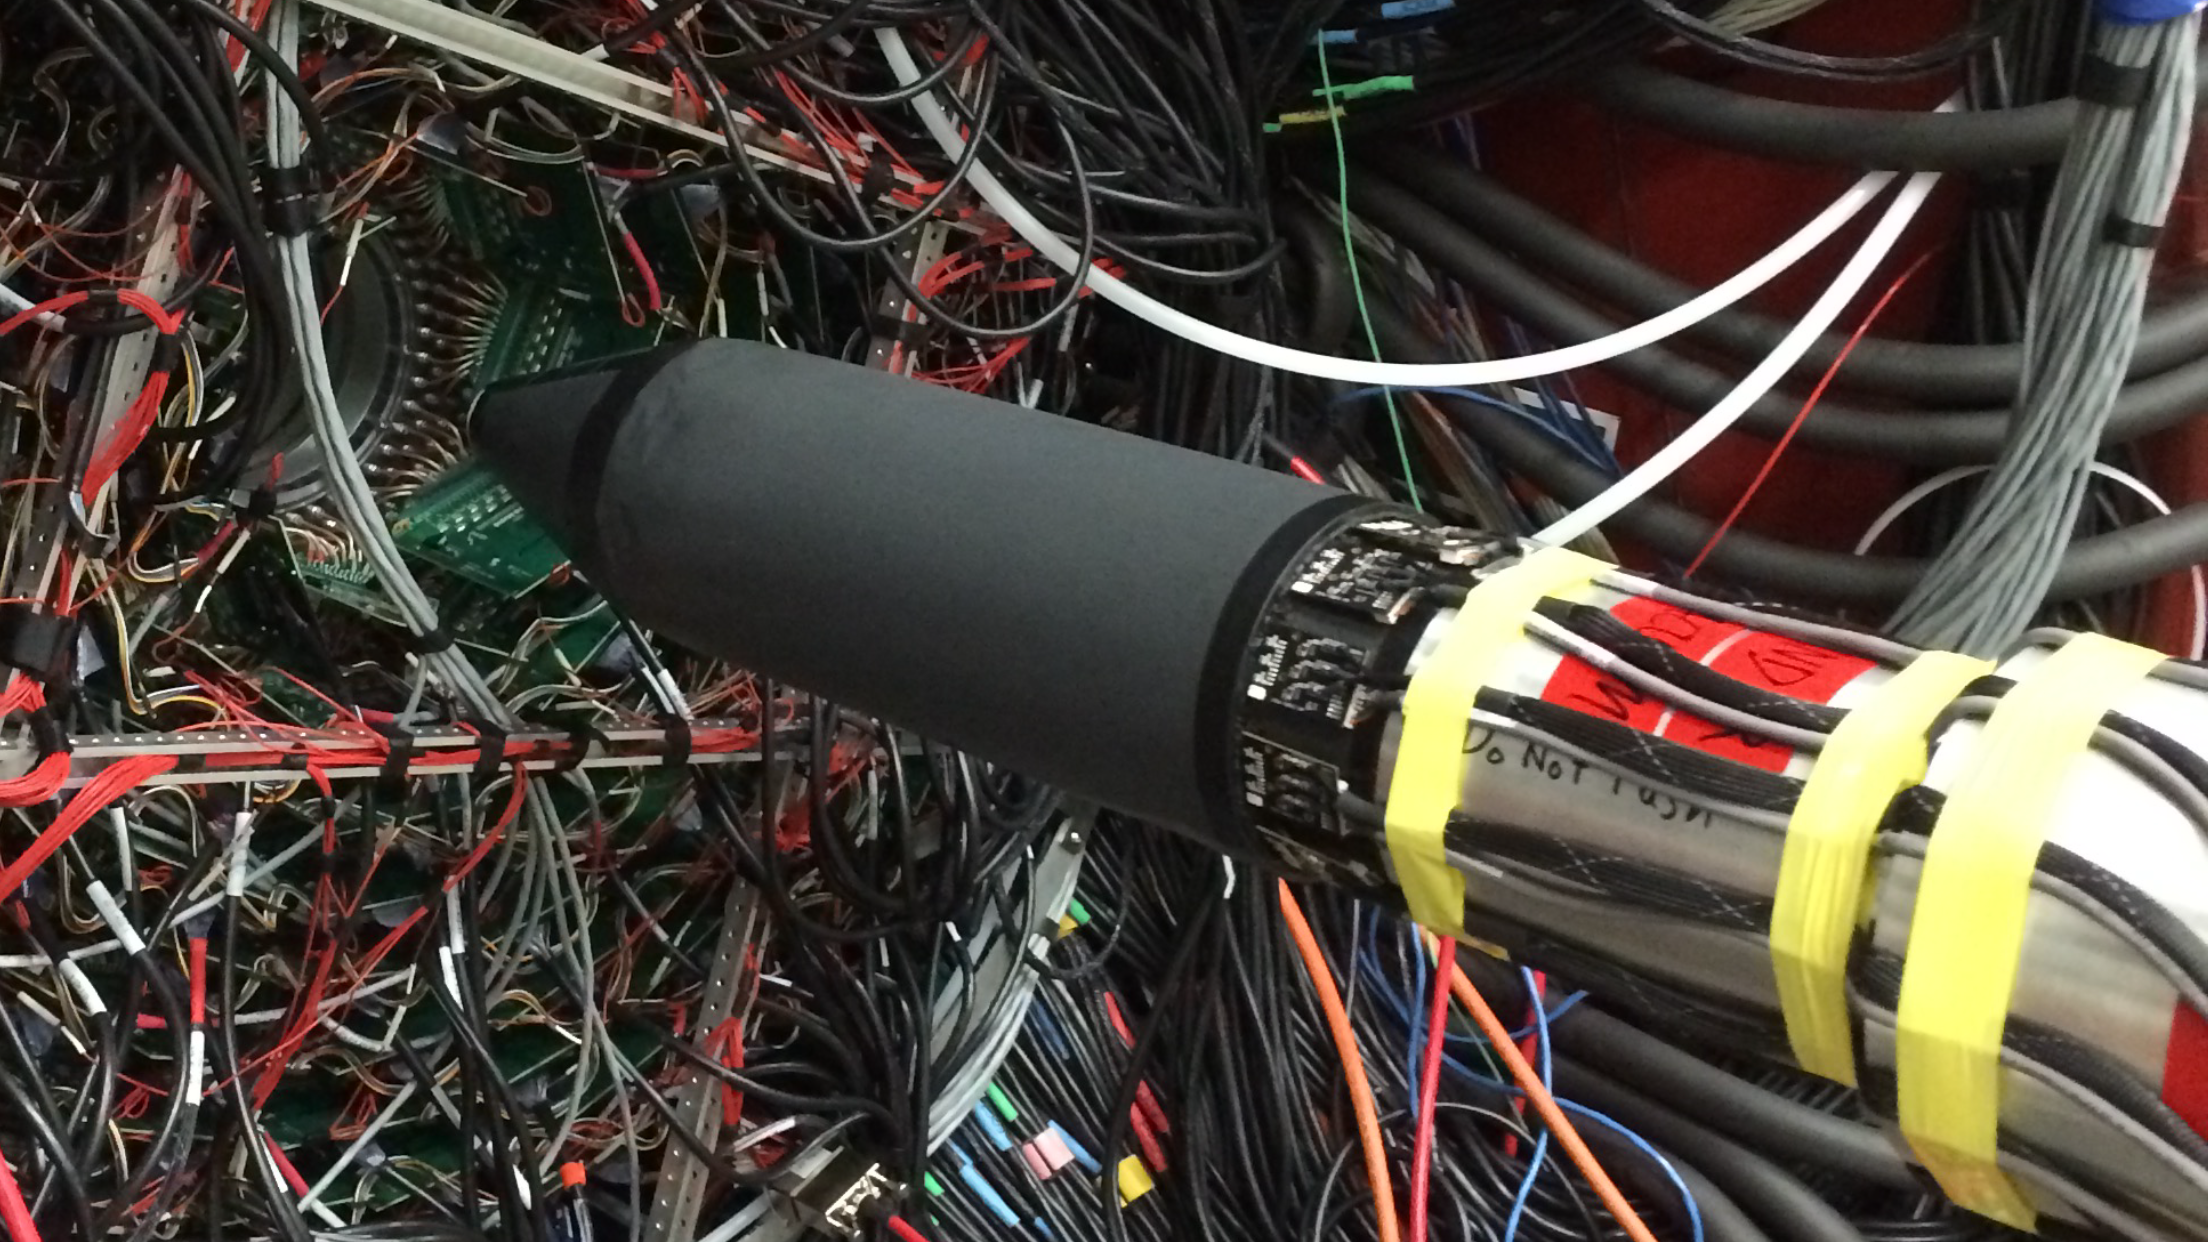
\includegraphics[width=1.0\columnwidth]{fabrication/figs/st_lt_v2}
	\caption{Light tight Start Counter mounted to the \gx{} liquid $\mathrm{H_{2}}$ target.  The beam direction is from right to left.  During operation the ST resides in the bore of the superconducting solenoid magnet which is visible in the top left corner.}
	\label{fig:light_tight_st}
\end{figure}
The tips of the inner and outer cones in the nose region were then taped together with electrical tape and trimmed of excess material. Furthermore, a cylindrical piece of Tedlar was taped down at the bend region and to the collar covering the ST1 boards.  The fully assembled and cabled ST mounted to the \gx{} liquid $\mathrm{H_{2}}$ target can be seen in Fig.~\ref{fig:light_tight_st}. 
%\section{GEANT4 Simulations} \label{sec:sim}

In this section, the Monte Carlo (MC) simulations that were conducted in order to better understand the performance and characteristics of scintillators machined to the nominal \gx{} Start Counter design are discussed.  Comparisons were made with the data observed in experiments conducted on the bench.  The MC studies were performed with the use of the simulation tool-kit GEANT4 which simulates the passage of particles through and interacting with matter \cite{geant4_website}.

\subsection{Simulating a Simplified Model of the ST} \label{sec:sim_simple}

As discussed in Sec.~\ref{sec:design_paddles}, the ST scintillator paddles have a unique geometry in which the nose section tapers in width as the paddles approach the beam line.  This tapering effect results in a unique phenomenon in which the light output of the scintillator paddle begins to increase as the source moves further away from the readout detector.  At first, this phenomenon is completely contrary to what one might expect. When the source moves further away from the end being readout, the photons have a larger effective path length and thus, have an increased probability in being lost for detection.  However, this is antithetical relative to what is observed.

A primitive GEANT4 simulation was conducted to investigate the aforementioned phenomenon. For simplicity, only the two trapezoidal regions of a machined scintillator paddle were considered.  Namely, the wide straight section and the tapered nose section which are illustrated in the GEANT4 event display  seen in Fig. \ref{fig:beam_off}.
	\begin{figure}[!htb]
	\centering
	\includegraphics[width=1.0\columnwidth]{simulation/figs/beam_off}
	\caption{Simulated straight \& nose section geometries.  Shown is the GEANT4 event display.  Left: wide straight section.  Right: tapered nose section.  The sections have been oriented such that they are in the same coordinate system as defined in HallD.  The yellow lines are the scintillator boundaries, while the red lines are the boundaries of the SiPM.}
	\label{fig:beam_off}
	\end{figure}  

The EJ-200 scintillator material ($\rho=1.023~\mathrm{g/cc^{3}}$, $n = 1.58$) \cite{ej200_specs} was simulated with only one free parameter utilized to characterize the scintillator bar \textit{i.e.}, the reflectivity of the \textit{G4LogicalSkinSurface}, was set to 98\% so there remained some finite probability that photons could be lost in the scintillator medium.  Furthermore, the SiPM readout detector was placed at the upstream end of the two sections, seen in Fig. \ref{fig:beam_off}.  Moreover, the SiPM was constructed as a \textit{G4SensitiveDetector} made of Silicon with a 100\% detection efficiency.  The SiPM was constructed to have an active area of $\mathrm{3 \times 12~mm^2}$ which is identical to the readout system described in Sec.~\ref{sec:design_sipms}.

In order to simulate a charged particle traversing through the scintillator medium resulting in the production of photons along its path through the material, optical photons were generated inside the volume of the simulated scintillator material.  The scintillation yield was defined to be $10,000 \gamma 's / $ 1 MeV \cite{ej200_specs}. For visual purposes, Fig. \ref{fig:100_events} shows 100 optical photons being produced at the tip of the far end of the two sections of the simulated scintillator paddle.
	\begin{figure}[!htb]
	\centering
	\includegraphics[width=1.0\columnwidth]{simulation/figs/100_events}
	\caption{100 Optical photons generated in the staight \& nose sections.  Left: wide straight section.  Right: tapered nose section.  The neon green lines are the paths of the optical photons.  It is clear that some photons do in fact escape the scintillator medium, while others are collected in the simulated SiPM detector.}
	\label{fig:100_events}
	\end{figure}

In order to sample the entirety of the two sections, 10,000 optical photons were generated at 16 different locations inside the medium of the scintillator. 
	\begin{figure}[!htb]
	\centering
	\includegraphics[width=1.0\columnwidth]{simulation/figs/gun_locations}
	\caption{Optical photon gun locations along the straight \& nose sections. Left: wide straight section.  Right: tapered nose section.  The magenta geometries indicate the scintillator boundaries of the two sections.  The red box is the sensitive SiPM detector, and the green cylinders represent the location of the 16 optical photon gun locations. The locations of the source were chosen to be equal distances apart relative to each of the two sections.}
	\label{fig:gun_locations}
	\end{figure}
The photon energies ranged between $0.5 - 3.0$ eV \cite{krane_ch7} and were generated randomly in $4\pi$ along a 3 mm path $(y-axis)$ in the scintillator medium.  The path was oriented orthogonal to the wide surface of the scintillator.  In essence, this simulates a charged particle traversing through the medium with a $\theta_{track} = 90^{\circ}$ in hall coordinates.  The number of photons collected by the SiPM at each of the 16 source locations is counted and correlated to the source location.  The results can be seen in Fig. \ref{fig:sim_results}.
	\begin{figure}[!htb]
	\centering
	\includegraphics[width=1.0\columnwidth]{simulation/figs/sim_results}
	\caption{Simulation results for simplified two section scenario. The total number of photons which were collected by the SiPM detector at each of the 16 source locations is plotted against the sources distance from the sensitive detector. Left: wide straight section.  Right: tapered nose section.}
	\label{fig:sim_results}
	\end{figure}
From the data it is clear that the geometry of the nose section results in an improvement of light collection as the source moves further away from the readout detector.  In fact, there is a factor $\approx 1/2$ light loss observed in the straight section upon comparing the number of hits collected at the closest and furthest locations relative to the readout detector.  However, there is factor $\approx 3/2$ light gain observed in the nose region.  These results are primarily due to the unique scintillator geometry.  This phenomenon is advantageous in the case of the ST since the majority of forward going charged particles will traverse through the nose region.

\subsection{Simulating Machined Scintillator Geometry} \label{sec:sim_mach}

Further simulations were conducted to simulate more realistically the effects of light collection that results from the ST scintillator geometry and optical surface quality.  The ST scintillator geometry was imported into GEANT4 from a Vectorworks CAD drawing utilizing the CADMesh utility \cite{cadmesh_g4} and is shown \textit{via} the GEANT4 event display in Fig. \ref{fig:pk_cadmesh}.
	\begin{figure}[!htb]
	\centering
	\includegraphics[width=1.0\columnwidth]{simulation/figs/pk_cadmesh}
	\caption{Scintillator geometry imported into GEANT4 utilizing CADMesh Utility.  The scintillator is  coupled to a SiPM detector.  Left: isometric view.  Right: top view.  The tapering of the nose section is clearly visible.}
	\label{fig:pk_cadmesh}
	\end{figure}
The SiPM was constructed as a $12 \times 12 \times\ 10\ \mathrm{mm^{3}}$ volume with a 100 $\mathrm{\mu m}$ air gap between it and the wide end of the straight section.  Furthermore, the volume surrounding the scintillator volume was air.  The EJ-200 scintillator material, SiPM silicon detector, and optical photons were defined in an identical manner discussed in Sec.~\ref{sec:sim_simple}.

To simulate the imperfections of the scintillator surfaces due to manufacturing and machining, an optical surface ``skin'' was defined.  The ``skin'' material was defined to be of they type ``dielectric-dielectric'' and made use of the UNIFIED physics model \cite{scint_surface_sim} to define an imperfect scintillator surface.  Both the transmission efficiency and reflection parameters were implemented as free parameters to study their various effects on light transmission..  

The UNIFIED model allows one to define the finish of the scintillator surface as \textit{polished}, \textit{ground}, or \textit{unified} and is illustrated in Fig.~\ref{fig:polished_vs_ground} \cite{scint_surface_sim}.
	\begin{figure}[tbph]
	\centering
	\includegraphics[width=1.0\columnwidth]{simulation/figs/polished_vs_ground}
	\caption{UNIFIED Model of scintillator surfaces.  Left: Polar plot of the radiant intensity of the polished (left) and ground (right) models.  Right: Polar plot of the radiant intensity in the UNIFIED model.}
	\label{fig:polished_vs_ground}
	\end{figure}

In the polished model, Fresnel reflection and refraction is assumed, where as the ground model allows for Lambertian reflection, Fresnel refraction, backscattering, as well as spike and lobe reflections.  The spike ($C_{ss}$) reflection parameter assumes the optical photons are reflected as if the surface was a perfect mirror.  The backscattering ($C_{bs}$) reflection parameter assumes the photon is reflected in the same direction of incidence.  The Lambertian ($C_{dl}$) reflection parameter assumes that the photons are reflected corresponding to a Lambertian distribution.  The lobe ($C_{sl}$) reflection parameter assumes that the photons will reflect based on the orientation of the micro-facet on the scintillator surface, where $\sigma_{\alpha}$ defined the standard deviation of the distribution of the micro-facets orientation \cite{scint_surface_sim}.  One caveat of the aforementioned models is that they assume identical parameters for the entire optical surface \cite{puneet_sim_wiki}.

As was done in section \ref{sec:sim_simple} 10,000 optical photons were generated in the scintillator medium every 2.5 cm and the number of hits collected in the SiPM were recorded.  The results of these simulations are show in Fig. \ref{fig:transm_eff_vs_sig_alpha}.
	\begin{figure}[!htb]
	\centering
	\includegraphics[width=1.0\columnwidth]{simulation/figs/transm_eff_vs_sig_alpha}
	\caption{UNIFIED Model results.  Left: polished model while varying the transmission efficiency.  Right: ground model with varying $\sigma_{\alpha}$ which characterizes the standard deviation of the surfaces micro-facet orientation.}
	\label{fig:transm_eff_vs_sig_alpha}
	\end{figure}
It is clear that while assuming a polished surface and the transmission efficiency is increased, the amount of light collected in the SiPM also increases.  This is illustrated in Fig.~\ref{fig:transm_eff_vs_sig_alpha}.  Similarly, as the number of micro-facet orientations increase, meaning a more coarsely ground surface, the amount of light collection in the SiPM decreases as expected.  Moreover, in the instances where the surface quality of the machined scintillators are good, the phenomenon of light increase in the nose region as the source moves further from the readout detector is clearly observed.


%\section{Calibration} \label{sec:calib}

In this section the various calibration procedures taken in order to minimize the time resolution and enhance both the particle identification (PID) and time of flight (TOF) capabilities of the Start Counter are discussed.

\subsection{Time-walk Correction} \label{sec:calib_tw}

The time-walk effect is a well understood consequence of leading edge discriminators (LED).  Analog signals of varying amplitudes crossing a fixed threshold, as determined by the discriminator threshold setting, will do so at varying times. %as illustrated in Fig.~\ref{fig:time_walk_effect}.
%	\begin{figure}[!htb]
%		\centering
%		\includegraphics[width=1.0\columnwidth]{calibration/figs/time_walk_effect}
%		\caption{Example of the time-walk effect. Three coincident analog signals A, B, \& C of varying amplitudes crossing a fixed threshold in a LED. The discriminator logic output signals vary in time relative to the amplitude of the incoming analog signal.  The signals shown above are simulated analog signals being fed into the LED's thus, they have negative polarity.}
%		\label{fig:time_walk_effect}
%	\end{figure}
Thus, the corresponding logic signal output from the LED will ``\textit{walk about}'' in time, resulting in an undesirable smearing of the measured ST TDC times.

The FADC250's provide a high resolution pulse time (62.5~ps/channel) that is time-walk independent\cite{pooser16}\cite{dong_fadc}.  
% WB here the question will come why bother with a discriminator then ?  
% EP I would argue the the mutihit capability (> number of FADC hits) and better resolution of the TDC's justify it's existance
Therefore, for events in which both the FADC and TDC register hits in the same channel, the pulse time can serve as a reference time for that event.  The TDC/FADC time difference is given by Eq.~\ref{eq:tdc_adc_tdiff} where $i$ is the paddle number index.
	\begin{equation} \label{eq:tdc_adc_tdiff}
		\delta t_{i} = t^{TDC}_{i} - t^{FADC}_{i}
	\end{equation}
	
The FADC250's return both the amplitude and integral of events which are above the programmed threshold \cite{dong_fadc}.  Since the amplitude better characterizes the rise time of the ADC pulse profile as compared to the pulse integral, it was selected for the time-walk corrections\cite{pooser16}.  Figure~\ref{fig:time_walk} (a) shows a typical time-walk spectrum, \textit{i.e.} $\delta t$ versus the pulse amplitude, for one paddle of the ST.
	\begin{figure*}[!htp]
		\centering
		\subfigure{\includegraphics[width=0.5\textwidth]{calibration/figs/before_tw_corr}}\hfill
		\subfigure{\includegraphics[width=0.5\textwidth]{calibration/figs/after_tw_corr}}
		\caption{Left: Single paddle time-walk spectrum; the line shown is the fitted function used to determine the correction factor. Right: post walk correction.  Plotted on the vertical axis is $\delta t$ and on the horizontal axis is the corresponding pedestal subtracted pulse amplitude spectrum.  }
		\label{fig:time_walk}
	\end{figure*}
This correlation is nonlinear and requires a functional form to describe it which is given by Eq.~\ref{eq:tw_corr_func_form} from Ref.~\cite{esmith_bcal}.
	\begin{equation} \label{eq:tw_corr_func_form}
		f^{w}_{i}\left(a/a^{thresh}_{i}\right) = c0_{i} + \frac{c1_{i}}{(a/a^{thresh}_{i})^{c2_{i}}}
	\end{equation}

In Eq.~\ref{eq:tw_corr_func_form} $f^{w}_{i}$ is the functional form of time-walk fit for the $i^{th}$ paddle, while $a$ and $a^{thresh}_{i}$ are the pulse amplitude and discriminator threshold converted to ADC units respectively.  Furthermore, $c0_{i}, c1_{i}, c2_{i}$ are the time-walk correction fit parameters.  This empirical function was chosen so that as the pulse amplitude increases, the correction function will asymptotically approach a constant, namely $c0_{i}$.  Therefore, at large pulse amplitudes the correction $f^{w}_{i}$ for $\delta t_{i}$ will reduce to an effective offset.  Moreover, signals with small amplitudes will have $\delta t_{i}$, corrected \textit{via.} $f^{w}_{i}$, so as to match the signals with large amplitudes.  Thus, signals of varying amplitude will exhibit a constant $\delta t_{i}$ as desired.
% WB what is the relation between \delta t_i  and f here. I think this would be useful 
% EP done.

The data in Fig.~\ref{fig:time_walk} (a) were fit using Eq.~\ref{eq:tw_corr_func_form} and ROOT's MINUIT $\chi^{2}$ minimization fitting library \cite{root_minuit} for pulse peak values ranging from [50, 2100].  An identical fit was carried out for each of the ST paddles.

% WB I would show the fitted function as illustration on the same graph
% EP Agreed, I was am on MK to provide the plots/fits

The most probable value (MPV) of the minimum ionizing peak, as observed \textit{via.} the pulse amplitude spectra, was chosen to be the location in which the time-walk correction is zero.  This location effectively serves as a reference point for the correction.  
% WB I would skip this
% EP done
%As seen in Fig. \ref{fig:pulsepeakch15} a ``pseudo'' MPV was utilized.
%	\begin{figure}[!htb]
%		\centering
%		\includegraphics[width=1.0\columnwidth]{calibration/figs/pulse_peak_ch15}
%		\caption{Typical pulse peak minimum ionizing distribution.  Shown is the pulse peak minimum ionizing distribution for paddle 3 during the Spring 2017 run. The red, vertical, dashed line in the histogram corresponds to the ``pseudo'' MPV ($a^{0}_{15}$) which was determined to be 500.}
%		\label{fig:pulsepeakch15}
%	\end{figure}
The MPV $(a^{0}_{i})$ was determined on a paddle by paddle basis by simply acquiring the pulse peak channel bin which had the most number of entries after the pulse peak channel 200.  The large spike in the pulse peak spectrum at very low pulse peak values are due to various electromagnetic background events clipping threshold and do not correspond to a true minimum ionizing particle traversing the scintillator medium.

Once the necessary time-walk correction parameters are determined, the correction is applied to the TDC time and is given by Eq. \ref{eq:tw_corr}.
	\begin{equation} \label{eq:tw_corr}
		T^{w}_{i} = t^{TDC}_{i} - f^{w}_{i}(a/a^{thresh}_{i}) + f^{w}_{i}(a^{0}_{i}/a^{thresh}_{i})
	\end{equation}
With the time walk corrections having been applied, the corrected timing distributions appear much more uniform in nature and exhibit a factor 1.75 improvement in resolution \cite{pooser16}.  Fig.~\ref{fig:time_walk} (b) illustrates the vast improvement in the time difference spectrum ($\delta t$) as a result of the applied time-walk corrections.
%	\begin{figure}[!htb]
%		\centering
%		\includegraphics[width=1.0\columnwidth]{calibration/figs/tw_dist_corr_ch15}
%		\caption{Time-walk corrected time difference spectrum.  Shown is the time-walk %corrected time difference spectrum for paddle 3 during the Spring 2017 run. The time-walk %corrected time difference spectrum has $\sigma_{\delta t_{15}} \approx 270 ps$}
%		\label{fig:twdistcorrch15}
%	\end{figure}
%Figure~\ref{fig:sttimeoverlaych15} illustrates the $\delta t_{15}$ distribution and the %relative effects of the aforementioned time-walk correction.
%	\begin{figure}[!htb]
%		\centering
%		\includegraphics[width=1.0\columnwidth]{calibration/figs/st_time_overlay_ch15}
%		\caption{Comparison of pre and post self-timing distributions.}
%		\label{fig:sttimeoverlaych15}
%	\end{figure}

\subsection{Propagation Time Corrections} \label{sec:calib_ptc}

As a charged particle traverses through the ST scintillator material the molecules become excited and a small fraction $(\approx 3\%)$ \cite{pdg_2012} of the excitation energy is released in the form of ``optical'' photons emitted uniformly in all directions.  Some photons will propagate along the scintillator by means of total internal reflection, some will escape the medium and be reflected back into the medium by virtue of the reflective Al foil wrapping, and some will be lost for detection by absorption and other mechanisms.  However, the majority of detected  photons will have undergone many total internal reflections while they propagated from their source to the SiPM detector placed at the upstream end.  The time between production in the ST scintillator paddles and detection is position dependent and must be accounted for as is discussed below.

The EJ-200 scintillator material has a refractive index of 1.58 \cite{ej200_specs} and the corresponding speed of light is $\approx \mathrm{19\ cm/ns}$.  However, what is measured in the lab is slower due to the fact that the majority of photons are not traveling in straight lines parallel to the medium boundaries. Instead they are constantly reflecting off the boundaries resulting in increased respective path lengths which contributes to the observed reduced velocity known as the effective velocity.  

Correcting for the time which light spends propagating in the scintillator material is a necessary correction since the ST paddles are 60~cm in length leading to a time difference of the order of 4~ns between photons produced in the tip of the nose and photons originating close to the upstream end where the SiPM resides.  Performing the propagation time corrections utilizing a common effective velocity is not the most optimal procedure for the case of the ST.  Studies performed with simulation and data showed that the unique geometry in the nose causes the effective velocity of light to be larger than that of the straight section and therefore they must be treated in an independent manner.

In order to conduct the propagation time corrections for the ST a distinct set of events needed to be selected so that a well defined reference time was being utilized.  This reference time was utilized as a measure of the event time for all other charged tracks intersecting the ST within the same event.  

For every charged track in a given event, two global tracking requirements were required.  First, only charged tracks with a good tracking confidence level were considered.  Secondly all charged tracks were required to have their vertex located within the target and radially within 1 cm from the beam. Only tracks passing these conditions were considered for analysis.  Further details regarding the event and track selection are found in Ref.~\cite{pooser16}.

%At least two specific tracks were required in each event in order to conduct the ST propagation time corrections.  One track that has hit the time of flight (TOF) detector and not the ST provides the reference time for that event.  All subsequent tracks were required to intersect the ST and not the TOF.  These tracks were used to provide the ST measure of the vertex time for that event.  This was done in order to avoid any potential bias in the calibration.  
	
% WB this is too detailed and technical. Refer to thesis and summarize the essential. From here to ...	
% EP done.

%The advantage of using the time associated with a track matched to the TOF is that the time resolution of the TOF is the best of any detector in Hall-D $(\approx 96\ \mathrm{ps})$ \cite{zihlmann_tof}. The calibrated (time-walk \& propagation) hit time returned by the TOF $(T^{TOF}_{hit})$ was then corrected for the flight time from the track vertex to the TOF $(T^{TOF}_{flight})$.  Equation~\ref{eq:tof_vertex_time} is the TOF measure of the track vertex time.
%	\begin{equation} \label{eq:tof_vertex_time}
%		T^{TOF}_{vertex} = T^{TOF}_{hit} - T^{TOF}_{flight}
%	\end{equation}

%In order to determine the time in which the beam bunch arrived at the interaction point ($T^{BB}_{vertex}$) the $T^{TOF}_{vertex}$ time must first be corrected for the RF measure of the vertex time ($T^{RF}_{vertex}$).  The steps required to correctly calculate $T^{BB}_{vertex}$ are discussed in detail in Ref.~\cite{pooser16}.  For every event, the first track satisfying the aforementioned fiducial track selection and is matched to the TOF will then have the associated $T^{BB}_{vertex}$ time calculated.  This time serves as the reference time for all other tracks that have intersected the ST in that event.

%The RF signal that is readout in Hall-D is provided by the CEBAF accelerator at a rate of 499 MHz (2.004 ns) while the beam bunches are produced at a rate of  249.5 MHz (4.008 ns).  The RF signal from the accelerator is multiplexed into TDC's however, the provided signal rate is too high to readout without causing overflow in the TDC buffers thus the RF signal is pre-scaled \cite{mattione_rf_wiki}.  The pre-scale factor was 128 and consequently the RF signal was readout every $\mathrm{128 \times 2.004\ ns = 256.512\ ns}$.  Thus, the time associated with the beam bucket that produced the event of interest must be calculated since it is not provided directly.

%For every event, the associated RF time is the pre-scaled time the RF signal arrived at the center of the target $(T^{RF}_{center})$. This time must be propagated out to the vertex location of the track since the photon responsible for the track spends a non-negligible finite amount of time traversing through the target before interacting with it. This propagation time $(T^{RF}_{prop})$ correction is given by Eq.~\ref{eq:rf_prop_time}
%	\begin{equation} \label{eq:rf_prop_time}
%		T^{RF}_{prop} = (z_{vertex} - z^{target}_{center}) \cdot \frac{1}{c} 
%	\end{equation} 
%Once the propagation time is summed with the centered RF time $(T^{RF}_{center})$ one obtains the measure of the RF time at the vertex of the track and is given by Eq. \ref{eq:rf_vertex_time}.
%\begin{equation} \label{eq:rf_vertex_time}
%	T^{RF}_{vertex} = T^{RF}_{center} + T^{RF}_{prop}
%\end{equation}

%Due to the inherent ambiguity associated with pre-scaling,  $T^{RF}_{vertex}$ is not the correct measurement of the time the beam bunch actually produced the track.  Therefore, one must ``step'' $T^{RF}_{vertex}$ to the time the track was produced as measured by $T^{TOF}_{vertex}$.  To do this one must first calculate the time difference $\delta T$ given by Eq. \ref{eq:rf_delta_t}.
%	\begin{equation} \label{eq:rf_delta_t}
%		\delta T = T^{TOF}_{vertex} - T^{RF}_{vertex}
%	\end{equation}
%Next, one must calculate the number of beam buckets $(N^{buckets}_{step})$ that have elapsed during the $\delta T$ time period and is given by Eq. \ref{eq:n_buckets_shift}, where $(N^{buckets}_{step})$ is rounded to the nearest integer.
%	\begin{equation} \label{eq:n_buckets_shift}
%		N^{buckets}_{step} = \frac{\delta T}{T^{BB}_{period}} = \frac{\delta T}{4.008\ ns}
%	\end{equation}
%Lastly one can now calculate the time the beam bunch arrived at the vertex that produced the track $(T^{BB}_{vertex})$ and is given by Eq. \ref{eq:bb_vertex_time}.
%	\begin{equation} \label{eq:bb_vertex_time}
%		T^{BB}_{vertex} = T^{RF}_{vertex} + T^{BB}_{period} \cdot N^{buckets}_{step}
%	\end{equation}

%For every event, the first track satisfying the aforementioned fiducial track selection and is matched to the TOF will then have the associated $T^{BB}_{vertex}$ time calculated.  This time serves as the reference time for all other tracks that have intersected the ST in that event.

% here

In order to properly calculate the propagation time ($T^{ST}_{prop}$) of photons produced by a charged track intersecting the ST, a few quantities must be known.  Particularly the time-walk corrected hit time ($T^{ST}_{hit}$), the flight time from the track vertex to the ST intersection point ($T^{ST}_{flight}$), and a well defined reference time corresponding to the event ($T^{BB}_{vertex}$).  With the reference time determined, all other charged tracks passing the previously discussed fiducial track selection and which have a match to the ST are analyzed.  Equation~\ref{eq:st_prop_time} illustrates the ST measure of the vertex time.
	\begin{equation} \label{eq:st_prop_time}
		T^{ST}_{prop} = T^{ST}_{hit} - T^{ST}_{flight} - T^{BB}_{vertex}
	\end{equation} 

This time difference is a direct measure of the amount of time the detected light produced by the intersecting charged track spent traversing the scintillator medium.  In order to perform the propagation time corrections the $z$-coordinate of the tracks intersection point with the ST $(z^{ST}_{hit})$ was also recorded for every charged track intersecting the ST relative to the upstream end.  However, $z^{ST}_{hit}$ only provides information of where the track intersected the ST along the $z$-axis and is not an accurate measure of the distance from the SiPM readout to the source of the scintillation light due to the unique ST paddle geometry.  This distance, $d^{ST}_{hit}$, was calculated for each for each $z^{ST}_{hit}$ directly while taking into account the paddle geometry. 

Once both $T^{ST}_{prop}$ and $d^{ST}_{hit}$ were calculated, the propagation correction calculation could be performed.  The calculated propagation times were then grouped into three distinct regions corresponding to the three unique geometrical sections of the ST namely the straight, bend, and nose regions.  These three regions were then fit utilizing a $\chi^{2}$ minimization technique with a linear function whose functional form is given by Eq. \ref{eq:pt_func_form} where the index $j$ indicates which region the fit is being performed relative to the $i^{th}$ paddle while $A$ and $B$ are the linear fit parameters.
	\begin{equation} \label{eq:pt_func_form}
	f^{i}_{j}(z) = A^{i}_{j} + B^{i}_{j} \cdot z
	\end{equation}
Figure~\ref{fig:proptimeuncorr} (a) illustrates the correlation between the two aforementioned quantities which has had an offset applied such that when $d^{ST}_{hit} = 0.0\ \mathrm{cm}$, $T^{ST}_{prop} = 0.0\ \mathrm{ns}$ and thus a well-defined correction could be applied across the full length of the paddle.
\begin{figure*}[!htb]
	\centering
	\subfigure{\includegraphics[width=0.5\textwidth]{calibration/figs/before_pt_corr}}\hfill
	\subfigure{\includegraphics[width=0.5\textwidth]{calibration/figs/after_pt_corr}}
	\caption{Left: Single paddle propagation time correlation.  $T^{ST}_{prop}$ is plotted on the vertical axis and $d^{ST}_{hit}$ is plotted along the horizontal axis. There is a clear correlation between the time in which optical photons are detected by the SiPM and the location of the scintillation light along the length of the paddle. Right: Single paddle propagation time after correction.}
	\label{fig:proptimeuncorr}
\end{figure*}

%The distributions and associated fits for the three regions are illustrated in %Fig.~\ref{fig:proptimeuncorrfits}.
%	\begin{figure}[!htb]
%		\centering
%		\includegraphics[width=1.0\columnwidth]{calibration/figs/prop_time_uncorr_fits}
%		\caption{Typical Start Counter propagation time projection correlation.  Left: Typical propagation time projection correlation for paddle 15 of the ST during the Spring 2015 run 2931.  The red line serves as a reference for the propagation time assuming it was a constant 15 cm/ns.  The magenta line is the fit corresponding to the straight section.  The green and dark blue solid lines correspond to the fits in the bend and nose section respectively.  Right: zoomed in view of data points.}
%		\label{fig:proptimeuncorrfits}
%	\end{figure}
	
With the fit parameters determined, an explicit time difference correction for each of the ST paddles could then be applied in order to calculate the ST measure of the vertex time given by Eq. \ref{eq:st_vertex_time}.
	\begin{equation}\label{eq:st_vertex_time}
	 	T^{ST}_{vertex}(z) = T^{ST}_{hit} - T^{ST}_{flight} - f^{i}_{j}(z)
	\end{equation} 
	
Figure ~\ref{fig:proptimeuncorr} (b) illustrates the propagation time corrected time as a function of the distance between the SiPM readout and the source of the scintillation light along the path of the ST paddles.
%\begin{figure}[!htb]
%	\centering
%	\includegraphics[width=1.0\columnwidth]{performance/figs/prop_time_corr}
%	\caption{Calibrated ST time versus the $z^{ST}_{hit}$ of charged tracks matched to the %ST.}
%	\label{fig:proptimecorr}
%\end{figure}
With the propagation time corrections applied it is clear that the ST time is no longer dependent on the where the charged track intersects with the paddles as expected.  The ST corrected time now provides an accurate measure of the vertex time for the track in the event and is discussed further in Sec.~\ref{sec:perform}.

\subsection{Attenuation Corrections} \label{sec:calib_ac}

%Photons propagating in a scintillator medium can be lost through scattering, absorption, or escape at the boundaries.  

The measured energy deposited $(dE_{M})$ from a charged particle traversing a scintillator medium is proportional to the number of photons created, which is in turn proportional to the integrated pulse read out by the FADC250. However, since the photons created \textit{via.} ionization can be lost through scattering, absorption, or escape at the boundaries as they propagate through the scintillator medium, the energy deposition measured by the SiPM does not correctly measure the energy deposited by the charged particle at the location of intersection with the scintillator and therefore must be corrected.

% WB this was already described above
% EP agreed.
% Photons produced in a scintillator medium, as a result of charged particles traversing through the material,  are subject to the property of total internal reflection.  If the resulting photons incident on the scintillator-air boundary have an angle of incidence which is smaller than the critical angle, then the photons will leave the scintillator medium and be lost for detection and thus contribute to the overall attenuation.  However, if the incident  photon has an angle of incidence which is equal to or greater than the critical angle, $39.3^{\circ}$ for the ST scintillator-air interface \cite{pooser16}, then those photons will totally internally reflect and may possibly be detected.  The photons that do in fact totally internally reflect however, are still subject to additional phenomena which contribute to the overall attenuation of photons in the scintillator medium.  

One can define an \textit{attenuation coefficient} which characterizes a particular materials ability to absorb photons. The attenuation coefficient is defined to be the length in the medium in which the initial number of primary photons are reduced by a factor of $1/e$ (36.8\%).  Since the loss of photons in scintillators equates to the loss of information relative to the event of interest, it is desirable to have a scintillator material with a long attenuation length.  For reference a flat $2 \times 20 \times 300\ \mathrm{cm^{3}}$ EJ-200 scintillator has a relatively long attenuation length on the order of 4~m \cite{ej200_specs}.

In order to determine the attenuation coefficients of interest, tracks hitting the ST which passed identical fiducial track selection cuts as discussed in Sec.~\ref{sec:calib_ptc}, were selected for analysis.  Furthermore, the tracks pedestal subtracted pulse integral (PI), track length inside the scintillator medium $(dx)$, energy deposition $(dE_{M})$, track momentum $(p)$, and the $z$-component of the tracks intersection point with the ST relative to the upstream end ($z^{ST}_{hit}$), where the SiPM is located, were recorded.  A plot of the uncorrected energy deposition per unit length versus the track momentum for tracks matched to the ST are shown in Fig.~\ref{fig:dEdx_vs_p}.  It is clear that no reliable PID can occur for tracks with $p > 0.6\ \mathrm{GeV/c}$.

%A plot of the uncorrected energy deposition per unit length versus the track momentum for tracks matched to the ST are shown in Fig.~\ref{fig:dEdx_vs_p_uncorr}.
%	\begin{figure}[!htb]
%	\centering
%	\includegraphics[width=1.0\columnwidth]{calibration/figs/ATT_UnCorr.pdf}
%	\caption{Typical uncorrected $dE/dx\ vs.\ p$ distribution in the Start Counter.  The ``banana band'' corresponds to protons while the horizontal band corresponds to  electrons, pions, and kaons.}
%	\label{fig:dEdx_vs_p_uncorr}
%	\end{figure}  
%It is clear that no reliable PID can occur for tracks with $p > 0.6\ \mathrm{GeV/c}$.

The pedestal corrected pulse integral (PI) data, normalized to the path length $dx$ of the track in the scintillator medium, were binned in 3.5~cm $z^{ST}_{hit}$ bins along the full length of the paddle. In order to properly quantify the amount of scintillation light created in the event, the most probable value (MPV) of the PI was extracted utilizing an empirical function which is both continuous and differentiable and is given by Eq.~\ref{eq:mpv} which utilizes three fit parameters namely $p_{0},\ p_{1},\ p_{2}$.
%These data in the nose section are represented in Fig.~\ref{fig:pisecnose}.
% WB these variations can also come from different track angles, the pulse integrals should be corrected by dx
% EP agreed
	\begin{equation}\label{eq:mpv}
	f(z)  = p_0 e^{(-p_1(z - p2))} \times (1+ \tanh(p_1(z - p2))) 
	\end{equation}
%In order to properly quantify this data, the most probable value (MPV) of the data was extracted utilizing the energy straggling distribution known as the Vavilov distribution \cite{vavilov_1957}.
%The Vavilov distribution, a generalization of the Landau distribution, is often utilized to describe the corresponding energy loss of charged particles traversing a thin layer of matter \cite{seltzer_1964}.  Unlike the more restrictive Landau distribution, the Vavilov distribution accounts for the maximum allowable energy transfer in a collision between a particle and an atomic electron \cite{schorr_1973}.  Therefore, the pulse integral data for each 1~cm bin along the the length of the ST paddles were fit utilizing the Vavilov distribution and the associated MPV was extracted.  
A fit to the data in a single 3.5~cm $z^{ST}_{hit}$ bin is illustrated in Fig.~\ref{fig:mpv_fit}. 
	\begin{figure}[!htb]
	\centering
	\includegraphics[width=1.0\columnwidth]{calibration/figs/mpv_fit}
	\caption{Pedestal subtracted pulse integral integral data normalized to the the track length in the scintillator medium for a single 3.5~cm bin along the paddle length.}
	\label{fig:mpv_fit}
	\end{figure}
Once the fits were successfully performed the MPV was extracted analytically and then plotted against the average value for each $z^{ST}_{hit}$ bin as seen in Fig.~\ref{fig:attfits}.
\begin{figure}[!htb]
	\centering
	\includegraphics[width=1.0\columnwidth]{calibration/figs/attn_fit}
	\caption{Fits to the attenuation data.}
	\label{fig:attfits}
\end{figure}
% With the above data in hand, one can quantitatively measure the attenuation of photons in the ST scintillators and is discussed below.

% WB these are piecewise CONTINUOUS !

As was discussed in Sec.~\ref{sec:sim_mach} the unique geometry of the ST is comprised of two distinct regions, \textit{i.e} the straight and nose sections.  These sections have differing properties in terms of light output and thus, time resolution.  Therefore, when performing attenuation corrections the two regions were treated independently in order to properly characterize photon attenuation.  It was empirically determined that the ideal fit function was piecewise continuous and follows Eq. \ref{eq:attn_fit_disc_pw} where the intersection (or correction boundary) of the two exponential fit functions was calculated ($Z^{i}_{b}$).
	\begin{equation} \label{eq:attn_fit_disc_pw}
	f_{c}^{i}(z) = 
	\begin{cases} 
		A^{i}_{S}e^{-B^{i}_{S} \cdot z} & z \leq Z^{i}_{b}\ \mathrm{cm} \\
		A^{i}_{N}e^{B^{i}_{N} \cdot z} + C^{i}_{N} & z > Z^{i}_{b}\ \mathrm{cm} \\
	\end{cases}
	\end{equation}
In Eq. \ref{eq:attn_fit_disc_pw}, the subscripts $S$ and $N$ denote the straight and nose sections respectively while $A^{i}, B^{i},$ and $C^{i}$ are the fit parameters for the $i^{th}$ paddle.  Exponential decay functions are typically used to describe the attenuation of photons in scintillator material.  However, for the unique case of the nose section, an exponential growth function was utilized.  It is clear from Fig.~\ref{fig:attfits} that the aforementioned exponential functions, corresponding to their respective geometrical sections, fit the data in a robust manner.
% WB I would skip the polynmial
% EP done.

Evaluating the fit function in the straight section at $z = 0\ \mathrm{cm}$ is representative of a minimum ionizing particle traversing through the upstream end closest to the SiPM readout.  In this instance the detected photons traverse through virtually no scintillator material, and are thus not subject to attenuation effects.  Therefore, for all charged particles passing trough the ST scintillator paddles we apply an attenuation correction factor $(R^{i}(z))$ to the deposited energy measurement per unit track-length $(dE_{M} / dx)$ to preserve the information regardless of where the track intersects the paddles. The corrected energy deposition per unit track length $(dE^{i}_{C}(z) / dx)$ for paddle $i$ is then given by Eq.~\ref{eq:de_corr_init} where the subscripts $C$ and $M$ are the corrected and measured quantities respectively. 
	\begin{equation} \label{eq:de_corr_init}
	\dfrac{dE^{i}_{C} (z)}{dx} = \dfrac{dE_{M}}{dx} \cdot R^{i}(z) = \dfrac{dE_{M}}{dx} \cdot \dfrac{f^{i}_{c}(0)}{f^{i}_{c}(z)}
	\end{equation}
	
Once all energy deposition measurements have had the appropriate attenuation corrections applied as was discussed above, the PID capabilities of the ST are considerably enhanced and are discussed further in Sec.~\ref{sec:perform}.
	
	
% WB there is a question: if we use the correct dEdX in MeV then it is not necessary to align all 'raw dE/dx' to a selected paddle but we fit the real dedx (as provided by PID knowlegde). This makes it dependent on existing calibation settings. 

% Then the part below is not necessary. 

% On the other hand when we use raw data, then we need to determine an overall scale factors to make sure the corrected raw dEdx is the same for all paddles. The expression below is in both cases not correct. I think this is one of the reasons we do not see a real improvement in dEdx.

% I would suggest we stay with raw data and do the additonal step and then are independent on energy calibrations. 

% It is required to note that paddle 15 was chosen as a reference paddle in an arbitrary manner.  Thus, for all tracks intersecting the full length of the ST we obtain the following relationship, seen in Eq.~\ref{eq:de_corr_final}, as desired.
%	\begin{equation} \label{eq:de_corr_final}
%	f^{i}_{c}(z) \cdot R^{i}(z) = A^{15}_{S}\ \forall\ z \in\ [0, 60]\ (cm)
%	\end{equation}
%
%Once all energy deposition measurements have had the appropriate attenuation corrections applied as was discussed above, the PID capabilities of the ST are considerably enhanced and are discussed further in Sec.~\ref{sec:perform}.

%\section{Performance} \label{sec:perform}

The Start Counter was installed in Hall-D just prior to the Fall 2014 \gx{} commissioning run.  It was not until the Spring 2015 commissioning run that enough statistics were obtained with an $\mathrm{LH_{2}}$ target to perform reliable calibrations.  With the aforementioned data set, the procedures to calibrate the detector and measure it's performance were developed and deployed.

As was discussed in previous sections, the geometry of the ST nose section results in an increase of the light output as the scintillation source moves towards the downstream end.  While investigating FADC250 data under nominal beam conditions, this phenomenon was immediately observed through the pulse amplitude and pulse integral data. Figure~\ref{fig:pippvszint} illustrates that similar to the bench measurements the light output increases exponentially, as the scintillation source moves towards the downstream end.
% WB one spectrum would probly be enought Amplitude or Pulse integral (here both look the same)
	\begin{figure}[!htb]
		\centering
		\includegraphics[width=1.0\columnwidth]{performance/figs/pi_pp_vs_zint}
		\caption{FADC spectra from the Spring 2017 run. Left: pulse integral versus the z-intersection of charged tracks matched to the ST. Right: pulse amplitude versus the z-intersection of charged tracks matched to the ST. The straight section corresponds to $40\ \mathrm{cm} < z < 80\ \mathrm{cm}$, the bend section $80\ \mathrm{cm} < z < 84\ \mathrm{cm}$, and the nose section $84\ \mathrm{cm} < z < 98\ \mathrm{cm}$.}
		\label{fig:pippvszint}
	\end{figure}
This feature of the ST geometry is quite advantageous since the majority of the charged tracks produced under the nominal \gx{} beam conditions intersect the ST in the nose region and therefore have the largest light amount of light collected by the SiPM's as the upstream end.

Once the proper attenuation corrections were applied to the data, the PID capabilities of the ST were greatly enhanced.  Figure ~\ref{fig:dEdx_vs_p_corr} illustrates the PID capability of charged tracks intersecting the ST.  As compared to Fig.~\ref{fig:dEdx_vs_p_uncorr}, the reliable separation of protons and other hadrons occurs for charged tracks with $p < 1.1\ GeV/c$ which is a factor two improvement from the uncalibrated data.
	\begin{figure}[!htb]
		\centering
		\includegraphics[width=1.0\columnwidth]{performance/figs/dEdx_vs_p_corr}
		\caption{Typical corrected $dE/dx\ vs.\ p$ distribution in the Start Counter.  Shown is the corrected $dE/dx\ vs.\ p$ distribution for tracks matched to the Start Counter in the Spring 2017 run. The ``banana band'' corresponds to protons while the horizontal band corresponds to charged electrons, pions, and kaons.  It is clear that pion/proton separation is achievable for tracks with $p < 1.1\ GeV/c$.}
		\label{fig:dEdx_vs_p_corr}
	\end{figure}  

After the previously discussed time-walk and propagation time corrections were complete, it was then possible to utilize the ST to measure the time of charged track vertices for tracks that are matched to the ST.  The vertex time is defined to be the time in which a polarized Bremsstrahlung photon interacted with the $\mathrm{LH_{2}}$ target and produced a charged track that intersected the ST.  An identical charged track selection process as outlined in Sec.~\ref{sec:calib_ptc} was utilized so that the time resolution of tracks matched to the ST could be measured.

The equation to calculate the ST measure of the vertex time is given by Eq.~\ref{eq:st_prop_time}.  In an identical manner outlined in Sec.~\ref{sec:calib_ptc}, $T^{RF}_{vertex}$ must be ``stepped'' to the time the charged track vertex was produced so as to obtain a proper measure of the RF time.  The resulting distribution in the time difference of these two times provides a measure of the ST time resolution and is seen in Fig. \ref{fig:beam_tof_corr_chan_15}.
	\begin{figure}[!htb]
		\centering
		\includegraphics[width=0.7\linewidth]{performance/figs/beam_tof_corr_chan_15}
		\caption[Typical Start Counter/RF time resolution distribution]{Typical Start Counter/RF time resolution distribution.  Shown is the time resolution distribution for sector 15 during the Spring 2015 run 2931. The x-axis is the time difference between $T^{ST}_{vertex}$ and $T^{BB}_{vertex}$. The blue histogram is the resolution in the straight section. The red and purple histograms correspond to the resolution in the bend and nose sections respectively. The black histogram is a sum of the three sections and corresponds to the resolution along the entire length of the paddle.}
		\label{fig:beam_tof_corr_chan_15}
	\end{figure}

The aforementioned fits were then carried out for each of the ST sectors with $\sigma$, and its associated error being calculated.  Then a weighted average of the 30 $\sigma$'s were calculated so that the ST could have its time resolution characterized in its entirety.  The same procedure was also conducted for the three individual sections.  Figure \ref{fig:timeresallinset} illustrates the uniformity in time resolution among all sectors of the ST.
	\begin{figure}[!htb]
		\centering
		\includegraphics[width=1.0\columnwidth]{performance/figs/time_res_all_inset}
		\caption{ST time resolutions as a function of sector number. The inset illustrates a 2~$\sigma$ Gaussian fit the the ST time minus the RF time. The resulting $\sigma$ of the fit provides a measure of the time resolution.}
		\label{fig:timeresallinset}
	\end{figure}

Figure \ref{fig:timeresallinset} indicates that the average time resolution of 300~ps is well below the design resolution of 350~ps.  Table \ref{tab:time_res_section} details the weighted average time resolution of all the ST sectors in the different geometrical regions.
\begin{table}[ch]
	\centering
	\begin{tabular}{|c|c|c|c|c|}
		\hline  \textbf{Section} & $\mathbf{\sigma_{all}}$ & $\mathbf{\sigma_{straight}}$ & $\mathbf{\sigma_{bend}}$ & $\mathbf{\sigma_{nose}}$ \\ 
		\hline $\mathbf{\sigma_{avg}}$ & 290 ps & 299 ps & 292 ps & 264 ps \\ 
		\hline 
	\end{tabular}
	\caption[Average time resolutions by section]{Average time resolutions by section. Shown is the average of all 30 ST sectors by independent geometrical regions.}
	\label{tab:time_res_section}
\end{table}
It is clear from Table \ref{tab:time_res_section} that what is observed is that measurements made with beam data exhibit the same phenomenon of substantial improvement in light collection, and thus time resolution, as light is produced further downstream in the nose region.

When these time resolution measurements were conducted with data collected in Spring 2017, approximately 3 years had elapsed since the paddles were first tested on the bench at FIU.  Prior experience with degrading scintillators indicates that degradation in time resolution will be visible in a matter of weeks.  However, after 3 years no degradation has been observed and the ST is still performing well below design resolution.
%\include{conclusions/conclusions}
%\include{acknoledgements/acknowledgements}
\endgroup

\section*{References}
\bibliography{bibliography/bibliography}

\end{document}